\documentclass{beamer}
\usepackage[utf8]{inputenc}
\usepackage[T1]{fontenc}
\usepackage[english]{babel}
\usepackage{amsmath, amssymb}
\usepackage{graphicx}
\usepackage{booktabs}
\usepackage{multirow}
\usepackage{xcolor}
\usepackage{hyperref}
\usepackage{tikz}
\usetikzlibrary{shapes.geometric}
\usepackage{adjustbox}

% Presentation theme
\usetheme{Madrid}
\usecolortheme{default}

% Custom colors
\definecolor{darkblue}{RGB}{0,102,204}
\definecolor{lightblue}{RGB}{173,216,230}
\definecolor{darkgreen}{RGB}{0,128,0}
\definecolor{lightgreen}{RGB}{144,238,144}
\definecolor{darkred}{RGB}{139,0,0}
\definecolor{lightred}{RGB}{255,182,193}

% Title information
\title{Conversational Toxicity Detection}
\author{Emanuele Fontana}
\institute{Università degli Studi di Bari Aldo Moro}
\date{}

\begin{document}

% Title slide
\frame{\titlepage}

\section{Introduction and Motivations}

\begin{frame}
\frametitle{Problem Statement and objectives}
\begin{block}{Key Challenges:}
\begin{itemize}
\item Online platforms harbor toxic interactions
\item Limited work on Italian language toxicity
\item Need for real-time detection capabilities
\end{itemize}
\end{block}
\begin{block}{Main Objective}
Developing systems for: 
\begin{itemize}
\item Toxic conversation detection
\item Personality classification (28 types)
\item Real-time toxicity detection 
\end{itemize}
\end{block}
\end{frame}

\section{Dataset}

\begin{frame}
\frametitle{Dataset Construction Pipeline}
\begin{columns}
\begin{column}{0.5\textwidth}
\textbf{Existing Toxic Dataset IDaToC:}
\begin{itemize}
\item Annotated Italian conversations
\item Various toxicity types
\item Emotional manipulation
\item Psychological violence
\end{itemize}

\vspace{0.3cm}
\textbf{Generated Non-Toxic Dataset:}
\begin{itemize}
\item Google Gemini API
\item Healthy conversations
\item 4 positive relationship types
\item Corpus balancing
\end{itemize}
\end{column}
\begin{column}{0.5\textwidth}
\begin{figure}
\centering
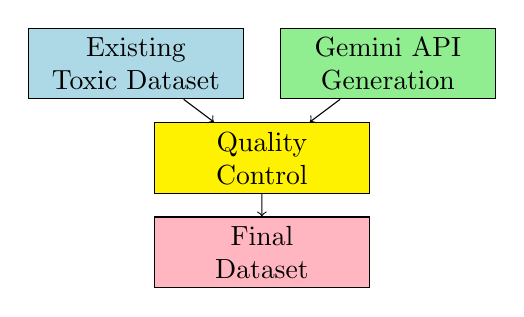
\begin{tikzpicture}[scale=0.8]
\node[draw, rectangle, fill=lightblue, text width=2.5cm, align=center] (existing) at (0,3) {Existing\\Toxic Dataset};
\node[draw, rectangle, fill=lightgreen, text width=2.5cm, align=center] (gemini) at (4,3) {Gemini API\\Generation};
\node[draw, rectangle, fill=yellow, text width=2.5cm, align=center] (quality) at (2,1.5) {Quality\\Control};
\node[draw, rectangle, fill=lightred, text width=2.5cm, align=center] (final) at (2,0) {Final\\Dataset};

\draw[->] (existing) -- (quality);
\draw[->] (gemini) -- (quality);
\draw[->] (quality) -- (final);
\end{tikzpicture}
\caption{Dataset generation pipeline}
\end{figure}
\end{column}
\end{columns}
\end{frame}

\begin{frame}
\frametitle{Dataset Generation Parameters}
\begin{itemize}
\item \textbf{Model}: Gemini-2.0-flash-lite - Fast inference with quality generation
\item \textbf{Temperature}: 1.8 - High creativity for diverse conversation styles
\item \textbf{Top-p}: 0.95 - Nucleus sampling for coherent text generation
\item \textbf{Top-k}: 40 - Limits vocabulary to most probable tokens
\item \textbf{Max tokens}: 2048 - Maximum conversation length per generation
\end{itemize}
\end{frame}

\section{Methodology}

\begin{frame}
\frametitle{Overall Approach}
\begin{columns}
\begin{column}{0.5\textwidth}
\begin{block}{Three Main Components}
\begin{enumerate}
\item \textbf{Binary Classification}: Traditional ML baseline
\item \textbf{Personality Classification}: Zero-shot + Fine-tuning
\item \textbf{Real-Time Detection}: Personality-based system
\end{enumerate}
\end{block}
\end{column}
\begin{column}{0.5\textwidth}
\begin{figure}
\centering
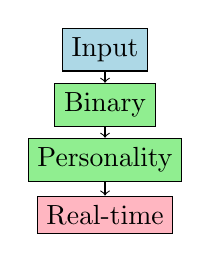
\begin{tikzpicture}[scale=0.7]
\node[draw, rectangle, fill=lightblue] (input) at (0,3) {Input};
\node[draw, rectangle, fill=lightgreen] (binary) at (0,2) {Binary};
\node[draw, rectangle, fill=lightgreen] (personality) at (0,1) {Personality};
\node[draw, rectangle, fill=lightred] (realtime) at (0,0) {Real-time};
\draw[->] (input) -- (binary);
\draw[->] (binary) -- (personality);
\draw[->] (personality) -- (realtime);
\end{tikzpicture}
\caption{Processing Pipeline}
\end{figure}
\end{column}
\end{columns}

\begin{block}{BERT Model}
\texttt{BERT-base-italian-xxl-cased} with 28 personality tokens
\end{block}
\end{frame}

\begin{frame}
\frametitle{Binary Classification}
\textbf{Compared Approaches:}
\begin{itemize}
\item \textbf{Approach 1}: Raw text + TF-IDF
\item \textbf{Approach 2}: Italian preprocessing + TF-IDF
\end{itemize}

\textbf{Italian Preprocessing Pipeline:}
\begin{itemize}
\item SpaCy (it\_core\_news\_sm)
\item Lemmatization
\item Stop words removal
\item Italian-specific tokenization
\end{itemize}

\textbf{Model Configuration:}
\begin{itemize}
\item Logistic Regression
\item Nested Cross-Validation (5-fold)
\item Hyperparameter grid search
\end{itemize}
\end{frame}

\begin{frame}
\frametitle{Personality Classification with BERT}
\begin{block}{BERT Model Enhancement}
\begin{itemize}
\item Base model: \texttt{dbmdz/bert-base-italian-xxl-cased}
\item Added 28 personality tokens: \texttt{[NARCISISTA]}, \texttt{[MANIPOLATORE]}, etc.
\item Extended vocabulary and embedding matrix
\item Context-aware personality detection
\end{itemize}
\end{block}

\begin{block}{Two Approaches Comparison}
\begin{columns}
\begin{column}{0.5\textwidth}
\textbf{Zero-Shot Learning:}
\begin{itemize}
\item No training required
\item Similarity-based classification
\item Uses personality descriptions
\item Cosine similarity matching
\end{itemize}
\end{column}
\begin{column}{0.5\textwidth}
\textbf{Fine-Tuning:}
\begin{itemize}
\item Task-specific training
\item Custom classifier head
\item [CLS] token representation
\item Dropout regularization (0.3)
\end{itemize}
\end{column}
\end{columns}
\end{block}
\end{frame}



\begin{frame}
\frametitle{Real-Time Detection System}
\begin{block}{Detection Mechanism}
\begin{itemize}
\item Message-by-message analysis
\item Context-aware predictions
\item Weighted confidence scoring
\item Adaptive threshold: 0.3
\item Immediate toxicity alerts
\end{itemize}
\end{block}
\begin{block}{Weighted Scoring Formula}
\begin{align}
\text{toxic\_score} &= \sum_{i=1}^{n} w_i \times \text{confidence}_i \\
\text{avg\_score} &= \frac{\text{toxic\_score}}{n} \\
\text{is\_toxic} &= \text{avg\_score} > 0.3
\end{align}
\end{block}
\end{frame}

\section{Experimental Results}

\begin{frame}
\frametitle{Binary Classification Results}
\begin{table}
\centering
\caption{Binary Classification Performance}
\begin{tabular}{lcccc}
\toprule
Approach & Accuracy & F1 & Precision & Recall \\
\midrule
Raw Text & 1.0000 & 1.0000 & 1.0000 & 1.0000 \\
Preprocessed & 1.0000 & 1.0000 & 1.0000 & 1.0000 \\
\bottomrule
\end{tabular}
\end{table}

\begin{alertblock}{Important Insight}
Preprocessing requires 20x more computational time without performance benefits
\end{alertblock}
\end{frame}

\begin{frame}
\frametitle{Personality Classification - Zero-Shot vs Fine-Tuned}
\begin{columns}
\begin{column}{0.5\textwidth}
\begin{table}
\scriptsize
\centering
\caption{Zero-Shot Performance}
\begin{tabular}{lc}
\toprule
Metric & Score \\
\midrule
Accuracy & 0.0268 \\
Macro Precision & 0.0010 \\
Macro Recall & 0.0364 \\
Macro F1-Score & 0.0020 \\
\bottomrule
\end{tabular}
\end{table}

\begin{figure}
\centering
\includegraphics[width=0.9\textwidth]{figures/confusion_matrix_zero_shot.png}
\caption{Zero-Shot Confusion Matrix}
\end{figure}
\end{column}
\begin{column}{0.5\textwidth}
\begin{table}
\scriptsize
\centering
\caption{Fine-Tuned Performance}
\begin{tabular}{lc}
\toprule
Metric & Score \\
\midrule
Accuracy & 0.5628 \\
Macro Precision & 0.5093 \\
Macro Recall & 0.5043 \\
Macro F1-Score & 0.5015 \\
\bottomrule
\end{tabular}
\end{table}

\begin{figure}
\centering
\includegraphics[width=0.9\textwidth]{figures/confusion_matrix_finetuned.png}
\caption{Fine-Tuned Confusion Matrix}
\end{figure}
\end{column}
\end{columns}
\end{frame}

\begin{frame}
\frametitle{Training Progress Analysis}
\begin{columns}
\begin{column}{0.6\textwidth}
\begin{figure}
\centering
\includegraphics[width=\textwidth]{figures/training_validation_loss_plot.png}
\caption{Training and Validation Loss Over Epochs}
\end{figure}
\end{column}
\begin{column}{0.4\textwidth}
\textbf{Training Details:}
\begin{itemize}
\item Early stopping after 15 epochs
\item Best validation loss: 0.2504
\item Dropout rate: 0.3
\item Learning rate: 1e-5
\item Patience: 10 epochs
\end{itemize}

\textbf{Performance Improvement:}
\begin{itemize}
\item \textcolor{darkred}{Zero-shot: 2.68\%}
\item \textcolor{darkgreen}{Fine-tuned: 56.28\%}
\item \textbf{21x improvement!}
\end{itemize}
\end{column}
\end{columns}
\end{frame}

\begin{frame}
\frametitle{Real-Time Toxicity Detection}
\begin{columns}
\begin{column}{0.5\textwidth}
\begin{table}
\centering
\caption{Real-Time System Performance}
\begin{tabular}{lc}
\toprule
Metric & Score \\
\midrule
Accuracy & 0.9884 \\
Precision & 0.9943 \\
Recall & 0.8889 \\
F1-Score & 0.9915 \\
\bottomrule
\end{tabular}
\end{table}

\end{column}
\begin{column}{0.5\textwidth}
\begin{figure}
\centering
\includegraphics[width=0.9\textwidth]{figures/confusion_matrix_realtime_weighted_score.png}
\caption{Real-Time Detection Confusion Matrix}
\end{figure}

\end{column}
\end{columns}
\end{frame}

\section{Conclusions}

\begin{frame}
\frametitle{Main Contributions}
\begin{block}{Key Results}
\begin{itemize}
\item \textbf{Binary Classification}: Perfect performance without preprocessing
\item \textbf{Personality}: Fine-tuning significantly outperforms zero-shot
\item \textbf{Real-Time}: 98.84\% accuracy in toxicity detection
\end{itemize}
\end{block}

\begin{block}{Innovations}
\begin{itemize}
\item First BERT-based system for Italian toxicity detection
\item Integration of personality classification + toxicity detection
\item Automatic pipeline for non-toxic data generation
\item Adaptive system with weighted scoring
\end{itemize}
\end{block}
\end{frame}

\begin{frame}
\frametitle{Limitations and Future Work}
\begin{columns}
\begin{column}{0.5\textwidth}
\textbf{Current Limitations:}
\begin{itemize}
\item Specific to Italian language
\item 28 personality framework
\item Limited context window (512 tokens)
\item Domain-specific dataset
\end{itemize}
\end{column}
\begin{column}{0.5\textwidth}
\textbf{Future Directions:}
\begin{itemize}
\item Multilingual extension
\item Larger datasets
\item GPT-based architectures
\item Real-world deployment
\item Extended context windows
\end{itemize}
\end{column}
\end{columns}

\vspace{0.5cm}
\begin{block}{Availability}
Code and dataset available on GitHub: \\
\url{https://github.com/Fonty02/NLP/tree/main/Exam}
\end{block}
\end{frame}

\begin{frame}
\frametitle{Thank You for Your Attention}
\begin{center}

\vspace{1cm}
\Large{Emanuele Fontana}\\
\normalsize{e.fontana7@studenti.uniba.it}

\vspace{0.5cm}
\normalsize{Università degli Studi di Bari Aldo Moro}
\end{center}
\end{frame}

\end{document}